%%
%% Template chap1.tex
%%

\chapter{Evaluation of Social Recommendation Systems}

We evaluate the algorithms implemented for this thesis in three ways. 

\begin{enumerate}
\item{\bf Live online user trials:} Our algorithms were made to tackle the problem of link recommendation on Facebook. Using various CF and SCF methods, we recommended links to users that have installed a Facebook App that was developed as part of this paper. The users rated each link on whether they liked or disliked the recommendation, and we collected these like/dislike ratings to evaluate the recommendation algorithms. A total of two trials was done, the first evaluates existing CF and SCF algorithms, and the second evaluates the new SCF algorithms developed for this paper.

\item{\bf Offline passive experiments:} Using the developed Facebook App, we were able to collect data over 30,000 Facebook users and their various interactions with each other on the Facebook network, as well as data on over 400,000 links. We evaluate the developed CF and SCF algorithms using this dataset on the problem of whether or not a user will have clicked \emph{``Like''} on a link. We show results here for various sets of training and testing data combinations.

\item{\bf User survey:} At the end of the first user trial, we conducted a user survey with the application users to evaluate their experiences with recommended links they were getting. We collected the responses to this survey and show how it reflects the results of the online and the offline experiments.

\end{enumerate}

\section{Facebook}

Facebook is a social networking service that is currently the largest in the world. As of July 2011 it had more that 750 million active users. Users in Facebook create a profile and establish ``friend" connections between users to establish their social network. Each user has a ``wall" where they and their friends can make posts to. These posts can be links, photos, status updates, etc. Items that have been posted by a user can be ``liked", shared, or commented upon by other users. 

\begin{figure}[h]
\centering
%\subfigure{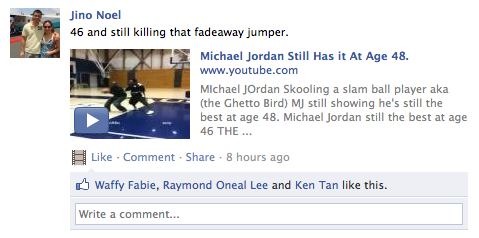
\includegraphics[scale=0.50]{img/posted-link.png}}
\subfigure{
\includegraphics[scale=0.50]{img/posted-link.eps}}

\caption{A link posted by the author that has been liked by three other users.}
\end{figure}

This paper seeks to find out how best to recommend links to individual users such that there is a high likelihood of them "liking" it. We do this by creating a Facebook application that recommends links to users everyday and the users could give their feedback on the links, whether they liked it or disliked it. 

\subsection{LinkR}
Facebook allows applications to be developed that can be installed by their users. As part of this project, the LinkR Facebook application was developed. The functionalities of the LinkR application are:

\begin{enumerate}
\item{Collect data that have been shared by users and their friends on Facebook.}
\item{Recommend links to the users daily.}
\item{Collect feedback from the users on whether they liked or disliked the recommendations.}
\end{enumerate}

\begin{figure}[h]
\centering
%\subfigure{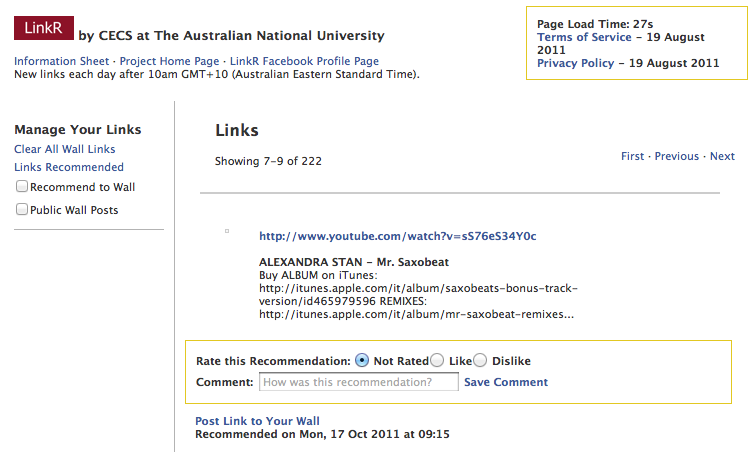
\includegraphics[scale=0.30]{img/linkr.png}}
\subfigure{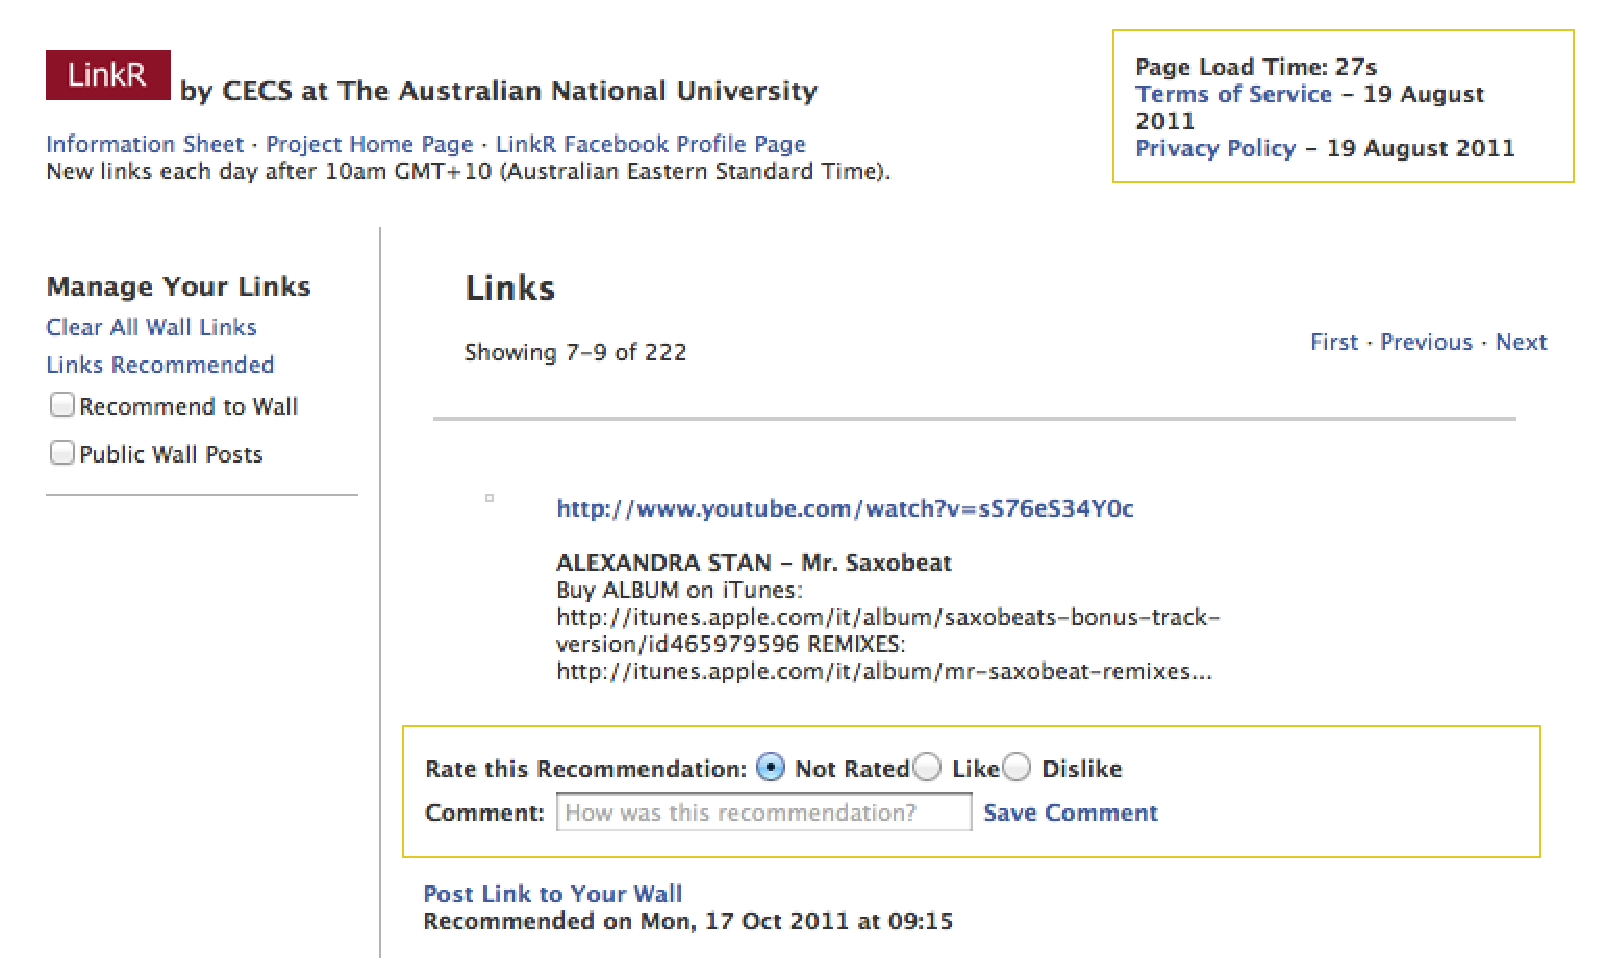
\includegraphics[scale=0.30]{img/linkr.eps}}
\caption{The LinkR application showing one of the recommendations.}
\end{figure}

The funding for the development, hosting, and maintenance of the LinkR application comes from a Google Research Award to the Australian National University (ANU) to study link recommendations on Facebook. The lead developer and maintainer of LinkR is Khoi-Nguyen Tran, a PhD student at the ANU. The algorithms it uses at the backend for recommendation were developed as part of this paper. 

\section{Dataset}

Using the LinkR Facebook application developed for this project, we were able to gather data on 34,245 users and 407,887 links.\footnote{As of October 18, 2011, 12:15am}

\subsection{User Data}

Data that are used for the user features are:
\begin{itemize}
\item {Gender}
\item {Birthday}
\item {$location\_id$}
\item {$hometown\_id$}
\item {Mapping of whether users $\x$ and $\z$ are friends on Facebook.}
\item {Interactions on Facebook between users $\x$ and $\z$. These interactions are used to build $\mathit{Int}_{\x,\z}$. } 
\end{itemize}

\subsection{Link Data}

Data that are used for the link features are:
\begin{itemize}
\item{$id$ of the user who posted the link.}
\item{$id$ of the user on whose wall the link was posted.}
\item{Description of the link from the user who posted it.}
\item{Link summary from the webpage.}
\item{Number of times the link has been liked.}
\item{Number of times the link has been shared.}
\item{Number of comments posted on the link}.
\item{List of users that have ``Liked" the link.}
\end{itemize}
Additionally, links that have been recommended by the LinkR application have the following extra features:
\begin{itemize}
\item{$id$'s of users who have clicked on the url.}
\item{Optional \emph{Like} or \emph{Dislike} rating of the LinkR user on the link.}
\end{itemize}

\subsection{Implicit Dislikes}
Outside of the \emph{Dislike} ratings that LinkR users give on recommended links, there is no other functionality within Facebook that allows users to explicitly define which links they do not like. Therefore, we needed some way to infer disliked links during training, to properly distinguish the links that users will like. We did this by considering links that were posted by the user's friends and which they have not ``Liked" as an example of a link that they do not like.

This is actually a big assumption as in a lot of cases given the nature of the Facebook News Feed and they may simply have not have seen the link, and may actually like the link if they had seen it. %Nevertheless, we find in our passive experiment and in live trial that this assumption is still useful.


\section{Evaluation Metrics}

\subsection{Mean Average Precision}

\begin{comment}
This paper uses a lot of different evaluation metric to compare the various algorithms discussed. For the collaboration recommendation algorithms which were run the MovieLens dataset, they were solving a regression problem so we used the Root Mean Squared Error (RMSE) metric which was also used to for the Netflix Prize competition.
\end{comment}

We define True Positives (TP) to be the count of relevant items that were returned by the algorithm, False Positives (FP) to be the count of non-relevant items that were returned by the algorithm, True Negatives (TN) to be the count of non-relevant items that weren't returned by the algorithm, and False Negatives (FN) to be the non-relevant items that were returned by the algorithm.

Precision is a measure of what fraction of items returned by the algorithm were actually relevant.

\[
Precision = \frac {TP} {TP + FP}
\]

For some problems, results are returned as a ranked list. The position of an item in the list must also be evaluated, not just whether the item is in the returned list or not. A metric that does this is Average Precision, which computes the precision at every position in a ranked sequence of documents. $k$ is the rank in a sequence of retrieved documents, $n$ is the number of retrieved documents, and $P(k)$ is the precision at cut-off $k$ in the list. $rel(k)$ is an indicator function equalling 1 if the item at position $k$ is a relevant document, and 0 otherwise. The average precision is calculated as

\[
AveP = \frac{\sum_{k=1}^n(P(k) \times rel(k))}{\text{number of relevant problems}}
\]

The main metric we use in this paper is the mean average precision (MAP). Since we make a recommendation for each user, these recommendations can be viewed as a separate problem per user, and evaluate the average precision for each one. Getting the mean of all the average precisions gives us an effective metric for the entire recommendation system.

\[
MAP = \frac{\sum_{u=1}^U AveP(u)}{\text{number of users}}
\]

\begin{comment}
\subsection{Other Metrics}

\[
RMSE = \sqrt{ \frac{\sum_{i=1}^N{ (r_i - p_i)}^2 }{N}}
\]

where {\bf r} are the true rating values for N movies and {\bf p} are the ratings predicted by the recommendation algorithms.

For the social recommendation algorithms, they are trying to solve a classification problem, so instead of RMSE we use various metrics such as accuracy, precision, recall, f1, and a variant of the Mean Average Precision.  Accuracy is a measure of how accurate the algorithm was in classifying all the items.

\[
Accuracy =  \frac{TP + TN}{TP + TN + FP + FN}
\]


Recall is the measure of what fraction of all relevant items items were actually returned by the algorithm.

\[
Recall = \frac {TP} {TP + FN}
\]

The F1 score is another measure of an algorithms accuracy, and is calculated as a weighted average between precision and recall.

\[
F1 = 2 \times \frac{precision \times recall}{precision + recall}
\]

The Area Under Curve (AUC) is equal to the probability that a classifier will rank a randomly chosen positive instance higher than a randomly chosen negative one. The AUC is related to the Gini coefficient (G1) and is defined as:

\[
G_1 = 1 - \sum_{k=1}^n(X_k - X_{k-1})(Y_k + Y_{k-1})
\]

\[
AUC = \frac{1 - G_1}{2}
\]

However among all these algorithms, MAP was the most applicable metric for the ranked link recommendations.
\end{comment}

\section{Training and Testing Data}

\subsection{Training Data}

Because of the sheer size of the Facebook data, it was impractical to run training and recommendations over the entire dataset. To keep the runtime of our experiments within reason, we used only the most recent four weeks of data for training the recommenders. Using only the four most recent weeks of data also alleviates temporal aspects of the user's changing preferences, i.e., what the user liked last year may not be the same as what he or she likes this year. We also distinguish between the three types of link likes/dislikes training data we can get from the dataset:

\begin{itemize}
\item {ACTIVE: The explicit ``Like" and ``Dislike" rating that a LinkR user gives on links recommended by the LinkR application. In addition to this, a click by a user on a recommended link also counts as a like by that user on that particular link. Only LinkR users will have this active data.}
\item {PASSIVE: The list of likes by users on links in the Facebook data and the inferred dislikes detailed above. All users in our dataset are included in this data.}
\item{UNION: Combination of the ACTIVE and PASSIVE data.}
\end{itemize}

\subsection{Live Online Recommendations}

For the recommendations made to the LinkR application users,  we selected for recommendation only links that the LinkR user has not like and has been posted only in the last two weeks. We recommend links only from the last two weeks because we consider recency to be a big issue. Older links have a greater chance of being about things that are outdated already, or worse, it may already be a broken link and not working anymore. In discussions before the start of the live user trials, we settled on recommending three links per day to the LinkR users. According to feedback from a survey done at the end of the first trial, three links per day was the most preferred number.

LinkR users were randomly assigned one of four algorithms in each of the two live user trials. The users were not informed which algorithm was assigned to them to remove any bias. We distinguish our recommended links into two major classes, links that were posted by the LinkR user's friends and links that were posted by users other than the LinkR user's friends. The LinkR users were encouraged to rate the links that were recommended to them, and even provide feedback comments on the specific links. In turn these ratings became part of the training data for the recommendation algorithms, and thus was used to improve the performance of the algorithms over time. The feedback options in LinkR are shown in Figure~\ref{fig:feedback}.

Based on the user feedback, we filtered out non-English links and links without any descriptions from the recommendations to prevent user annoyance.

At the end of the first trial, we conducted a user survey with the LinkR users to find out how satisfied they were with the recommendations they were getting.

\begin{figure}
\centering
%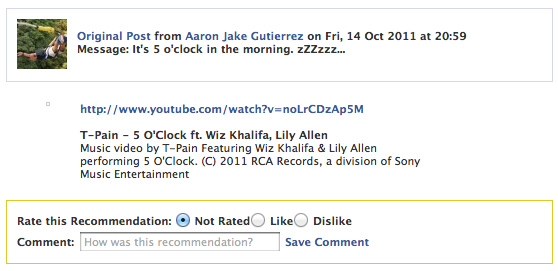
\includegraphics[scale=0.5]{img/linkr_rating.png}
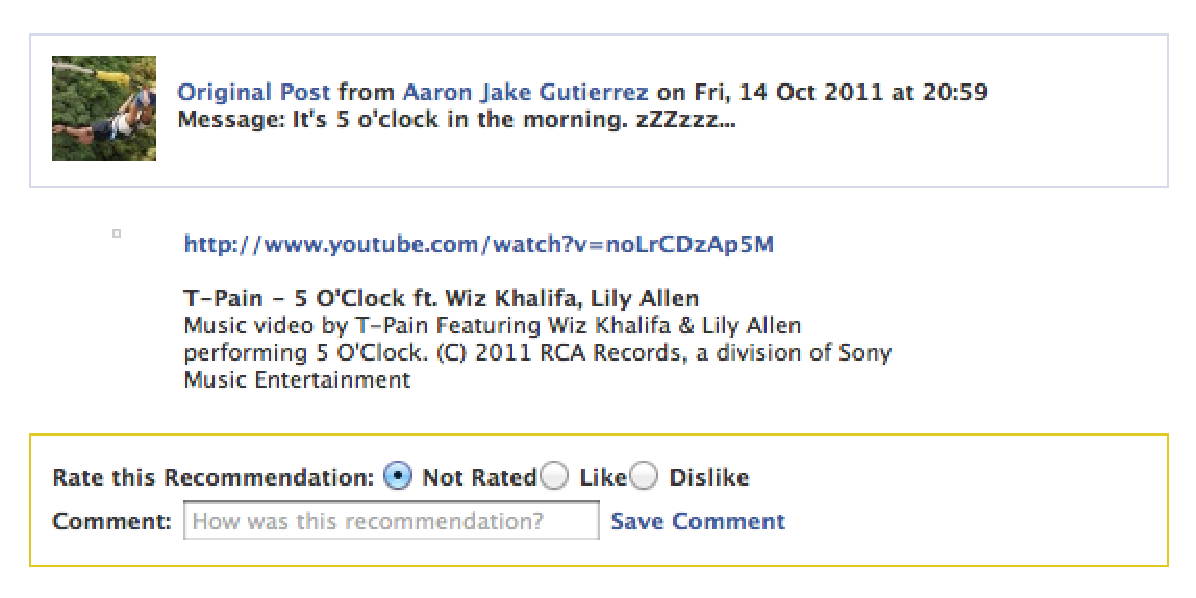
\includegraphics[scale=0.5]{img/linkr_rating.eps}
\caption{Screenshot of a recommendation made by the LinkR application with the rating and feedback options.}
 \label{fig:feedback}
\end{figure}

 
\subsection{Test Data}

Similar to our selection for training data, the test data used for our passive experiment also uses only the most recent 4 weeks of data. We distinguish the test data into the following classes:

\begin{itemize}
\item{FB-USER-PASSIVE: The PASSIVE like/dislike data for all Facebook users in the dataset.}
\item{APP-USER-PASSIVE: The PASSIVE like/dislike data for only the LinkR application users.}
\item{APP-USER-ACTIVE-FRIENDS: The ACTIVE like/dislike data for the LinkR users, but only for friend recommended links.}
\item{APP-USER-ACTIVE-NON-FRIENDS: The ACTIVE like/dislike data for the LinkR users, but only for non-friend recommended links.}
\item{APP-USER-ACTIVE-ALL: The entire active like/dislike data for the LinkR users.}
\end{itemize}

During passive experiments, we simply select which combination of training data and testing data to use. This helped us see which training-test data combination best reflected the results of the live trials. %Eventually, it was found that using UNION data for training and testing on APP-USER-ACTIVE-ALL best reflected the results of the live trials. 
In cases where training and testing data overlap, i.e., training on PASSIVE and testing on APP-USER-PASSIVE, we get a random 20\% subset of the training data per user for testing. These links are then removed from the training data to ensure that there are no common links between the training data and the test data.

In this chapter we have discussed how we are going to evaluate the CF and SCF algorithms we describe in the next two chapters: An online live trial of Facebook users who have installed the LinkR application, offline passive testing using the various training data and testing data combinations and evaluated using the mean average precision metric, and finally a user survey conducted with the LinkR users at the end of the first live user trial.

In the next chapter we evaluate existing CF algorithms and one extensions to SCF algorithms we have made and see which one performs best on all three evaluation phases.